
\chapter{Methodology}
\label{cpt:methodology}

\section{Sample Extraction}
\label{sec:methodology:sample_extraction}

\todo{Add references}
As simulators have become standard tools in computer architecture research, we have seen an increase in complexity of the simulated systems. 
From simulators supporting functional models of an in-order single core processor to detailed simulations of multicore out-of-order processors.
The increased complexity implies that the work done per simulated instruction has increased.
In addition, as simulation has become a standard tool the benchmarks simulated has shifted from simple micro-benchmarks to actual consumer applications. 
Even though we have observed an increase in available processing power alongside this complexity increase, it has proved insufficient to offset the slowdown of more advanced simulators.
With this development, it is no longer feasible to simulate a benchmark start to finish.

In order to keep the simulation time at acceptable values, researchers often extract samples from a benchmark that they simulate in full detail. 
Instructions up to this sample point are simulated using less detail in order to save time.
The selection method used to select this sample can significantly affect the outcome of the simulation.
In this section, we cover three methods for selection samples, one of which we will use in our experiments.

\todo{Rewrite everything below}

\subsection{Naive Approch}
A naive approach for extracting excerpts from benchmarks is to specify a number of cycles into the execution where the excerpt starts, in addition to the length of the excerpt.
The reason an excerpt does not usually start at the first executed instruction is because of the startup effect.
When an application starts, it usually performs some initialization tasks before the main routines of the application starts.
During this startup phase, the application may not behave as it will during the remainder of its execution.
As a result, simulating this startup phase might yield unexpected results that are not representative for the benchmark as a whole.
The problem with the naive approach to extracting excerpts is that it is hard to define an offset, and then guarantee that this offset is sufficiently large to skip the startup phase for all benchmarks.

\subsection{SMARTS}

\subsection{SimPoint}
More sophisticated approaches to this problem include tools that analyze the instruction stream of a benchmark as it executes.
Based on this analysis the tool will attempt to locate one or more intervals that based on a selected metric can be considered representative for the entire benchmark execution.
SimPoint\cite{Hamerly2005} is one such tool, based on Pin~\cite{Luk2005}.
Put simply, SimPoint will analyze the benchmark code and divide it into basic blocks.
A basic block is a group of instructions with only a single entry point, the first instruction, and a single exit point, at the last instruction.
It wil then analyze the running program, and each execution interval is classified using a Basic Block Vector (BBV)
The BBV contains an entry for each basic block in the program and a counter indicating how many times the interval executed this block.
After classifying all intervals, SimPoint uses K-means clustering to create K groups of intervals that have similar BBVs.
Within each cluster, the interval closest to the cluster center is selected to represent the cluster. 
The output of SimPoint is the start and length of each cluster's representative interval, along with a weight indicating how much of the entire program execution this cluster represents.

Previous work by Hamery~et~al.~\cite{Hamerly2004} has compared the simulation results of SimPoint selected intervals and intervals selected by the naive approach to the results of simulating the entire benchmark.
When using SimPoint selected intervals each interval is simulated independently, and a weighted sum of simulation results is created using the generated weights.
Hamerly~et~al. show that using SimPoint selected intervals can improve the accuracy of the simulation results. 
They also show that the value of K, the number of intervals returned, and the length of the interval effect the accuracy of the solution. 

\todo{Extend the last sentence with some actual results from the Hamerly et al. paper}

\begin{figure}
\centering
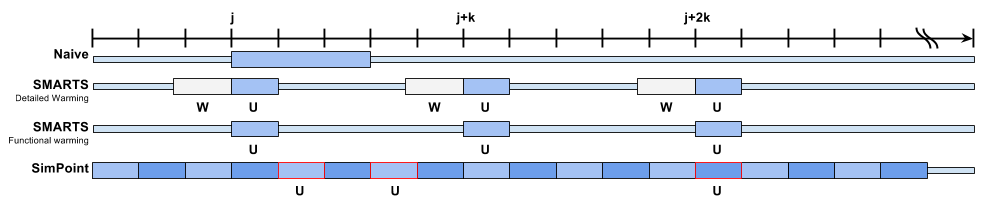
\includegraphics[width=\textwidth]{figures/methodology/sample_extraction_tools}
\caption{TODO}
\todo{Not readable when printed, have to fix text sizes}
\label{fig:background:simpoint:sampleextract}

\end{figure}

\section{Base Experiment}
\todo{Describe base experiment with locked L2 size, L3 depending on workload size. All workloads executed. Define speedup, define STP. Define HMS. Quickly explain why we need both STP and HMS, what differences may they show? Also mention that we capture number of misses (and miss rate). Explain when we dump statistic snapshots for each benchmark, and that we restart benchmarks during simulation.}

\section{L2 Sensitivity}
\todo{Explain how we repeat the base experiment above with varying L2 size, but all other parameters locked. Explain how results of these experiments are compared the base experiment using changes in the already presented metrics.}

\section{Simulator Parallelism Sentitivity}
\todo{Explain how we repeat the base experiment but this time vary the quantum of the clock skew minimization barrier. This result will give an indication of how much this variable affects our results. As we are not comparing against real HW or even a proven cycle accurate simulator, these results only give an indication and cannot be used to draw a conclusion. If we show a large variation, we do have something to write about in the discussion and something to add to future work.}

\todo{It is natural to use to relative change in one of our existing metrics when comparing, we should also mention the simulation time differences, but they do not need to be plotted.}

\todo{The effect of clock skew minimization is discussed in T. Carlson et al. 2011}

\todo{We will only investigate barrier synchronization, the other option, random pair synchronization, is expected to give a higher performance, but also is expected to give a higher clock variance.}

\begin{table}[ht]
\centering

\begin{tabular}{r}
\textbf{Quantum Size} \\ \hline
1 cycles \\
10 cycles \\
100 cycles \\
1000 cycles
\end{tabular}
\caption{Barrier synchronization quantum sizes}

\todo{I picture one cycle may be problimatic}

\end{table}